\chapter{Literaturübersicht}
\label{kap:literaturübersicht}
Die nachfolgende Literaturübersicht soll einen Überblick über relevante Projekte und Visualisierungen schaffen, welche sich insbesondere mit Zugverspätungen und dessen Auswirkungen innerhalb eines Zugnetzwerks befassen. Nebst den visuellen werden auch algorithmische Verfahren, insbesondere zur Erkennung von Mustern, betrachtet.

\section{Visualisierungs-Pipeline}
\textbf{Dashboards} sind ein effektives Werkzeug, um grosse Mengen an Daten verständlich und auf einen Blick darzustellen. Um ein qualitativ hochwertiges Dashboard zu erstellen, müssen sowohl die Daten und Algorithmen als auch die Visualisierungen und Interaktionen aufeinander abgestimmt sein. Um das Zusammenspiel dieser Komponenten zu veranschaulichen, werden häufig \textbf{Visualisierungs-Pipelines} verwendet (siehe Abbildung \ref{fig_pipeline_traffic_visualization}).

\begin{figure}[H]
    \caption{Visualisierungspipeline für Verkehrsdaten \parencite[S. 2971]{survey_traffic_data_visualization_2015}}
    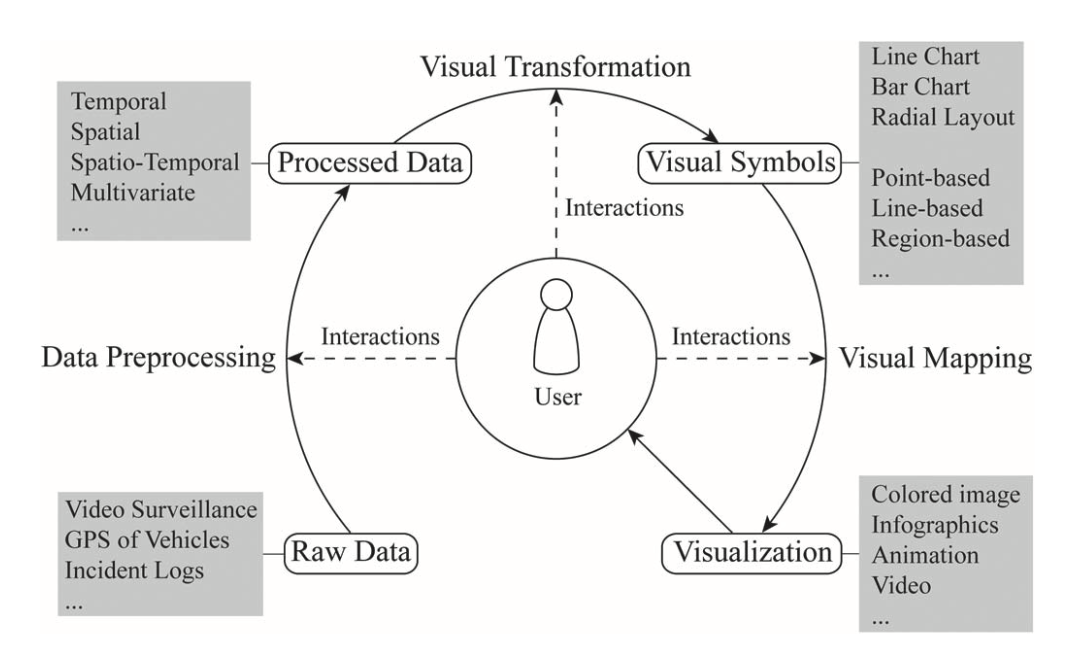
\includegraphics[width=.8\linewidth]{content/00_assets/traffic_visualization_pipeline.png}
    \label{fig_pipeline_traffic_visualization}
\end{figure}

Das Paper von Chen et al. betrachtet beispielsweise verschiedene Visualisierungen zum Thema Verkehrsdaten anhand einer solchen Pipeline. Eine Visualisierung über Verkehrsdaten durchläuft gemäss Chen et al. vier verschiedene Phasen. In der Phase \textit{Raw Data} werden die Daten erfasst. Dies geschieht meist über Sensoren, GPS oder Log-Aufzeichnungen der Geräte. Anschliessend werden die Daten im \textit{Data Preprocessing} entsprechend aufbereitet. Im Rahmen des Data Preprocessing werden Datenfehler und Ausreisser entfernt. Aufgrund der grossen Datenmengen, welche bei Verkehrsdaten auftreten, ist es wichtig, dass diese Daten effizient gespeichert werden. Dies geschieht über \textit{Datenaggregationen} und die richtige Wahl eines effizienten \textit{Datenverwaltungssystems}. Das Ergebnis des Data Preprocessing ist ein Datensatz mit sowohl räumlichen, zeitlichen als auch multivariaten Informationen. Durch \textit{Visual Symbols} werden die Daten dem Nutzer mithilfe von unterschiedlichen Visualisierungen (bspw. Liniendiagramm) dargestellt. Um das Verständnis der Daten noch weiter zu fördern, werden im Schritt \textit{Visual Mapping} visuelle Variablen verwendet. \textbf{Visuelle Variablen} erlauben es bspw. die Grösse oder Farbe von Visualisierungen an die Daten zu koppeln \parencite[S.2971]{survey_traffic_data_visualization_2015}. 

Ein Beispiel hierfür ist das Projekt \textit{Trains in Time} (siehe Abbildung \ref{fig_trains_in_time}). Hier werden die visuellen Variablen Grösse und Farbe verwendet, um die Zugverspätung und Zugauslastung im Pariser Streckennetz zu visualisieren. Die Farbe repräsentiert hierbei die Verspätung und die Grösse der Kreise die Auslastung eines Zuges \parencite{trains_of_data_2012}.   

\begin{figure}[H]
    \caption{Trains in Time \parencite{trains_of_data_2012}}
    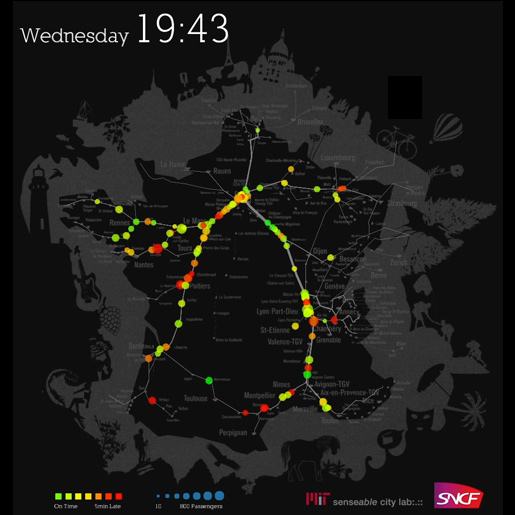
\includegraphics[width=.5\linewidth]{content/00_assets/trains_in_time.jpg}
    \label{fig_trains_in_time}
\end{figure}

Ein weiteres Beispiel für die Verwendung von visuellen Variablen ist das Dashboard von Dimanche et al. (siehe Abbildung \ref{fig_massive_railway_visualization}). Dieses Dashboard richtet sich primär an Experten und erlaubt es, das Pariser Zugverkehrsnetzwerk zu explorieren. Die Züge werden hierbei als Rechtecke visualisiert. Die Breite des Rechtecks entspricht der Fahrzeit, die Länge entspricht der zurückgelegten Strecke und die Farbe widerspiegelt die Verspätung \parencite{visualization_tool_operating_experts_2017}.

\begin{figure}[H]
    \caption{Visualisierung von einzelnen Zügen und deren Verspätungen \parencite[S. 15843]{visualization_tool_operating_experts_2017}}
    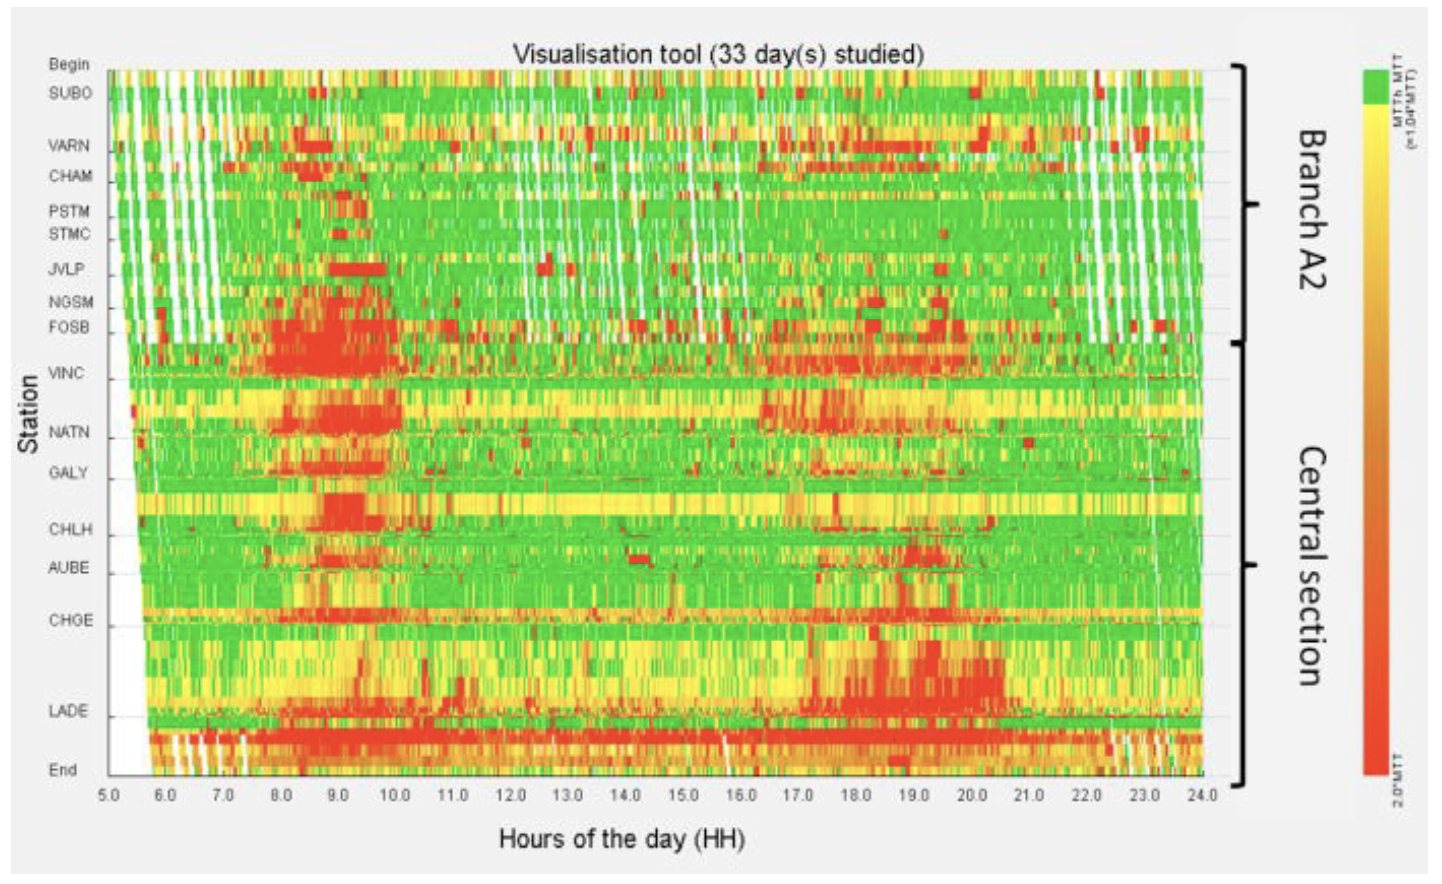
\includegraphics[width=.5\linewidth]{content/00_assets/massive_railway_visualization.png}
    \label{fig_massive_railway_visualization}
\end{figure}

Die Visualisierungs-Pipeline selbst wird nicht einmal durchlaufen, sondern ist ein wiederkehrender Zyklus. Der Nutzer kann mithilfe von Interaktionen Einfluss auf diverse Aspekte dieses Zyklus nehmen. So kann er bspw. durch Filtereinstellungen die Datenmenge reduzieren oder mithilfe von entsprechenden Parametern direkten Einfluss auf die Funktionsweise der dahinterliegenden Algorithmen nehmen \parencite[S.2971]{survey_traffic_data_visualization_2015}.

\section{Dashboard Visualisierungen}
Wie bereits angesprochen sind Dashboards eine beliebte Option, um komplexe und grosse Datenmengen zu visualisieren. Ein Dashboard erlaubt es, unterschiedliche Sichten auf den gleichen Datensatz zu erhalten. Dies geschieht mithilfe von unterschiedlichen Visualisierungen. Jede Visualisierung veranschaulicht hierbei einen anderen Aspekt der Daten. Visualisierungen sind keine Momentaufnahme, sondern interaktive Sichten auf Daten. Der Nutzer kann bspw. mittels Filtereinstellungen Einfluss auf das finale Aussehen einer Visualisierung nehmen. Auch können die Visualisierungen mithilfe von Brushing und Linking Verfahren «verbunden» sein. 

Ein Beispiel für ein Dashboard, welches unterschiedliche Sichten ermöglicht, ist das Dashboard von Jeph et al. (siehe Abbildung \ref{fig_raildash}). Ihr Dashboard visualisiert den Einfluss von grossen Ereignisse auf den Zugverkehr in Tokyo sowie auf das Laufverhalten von einzelnen Personen. Hierbei wurden grosse Mengen von Smartphone-GPS-Daten, Daten über Ereignisse und Events, sowie Zugnetzwerkdaten kombiniert \parencite{raildash_2022}.

\begin{figure}[H]
    \caption{Raildash Dashboard \parencite[S. 93]{raildash_2022}}
    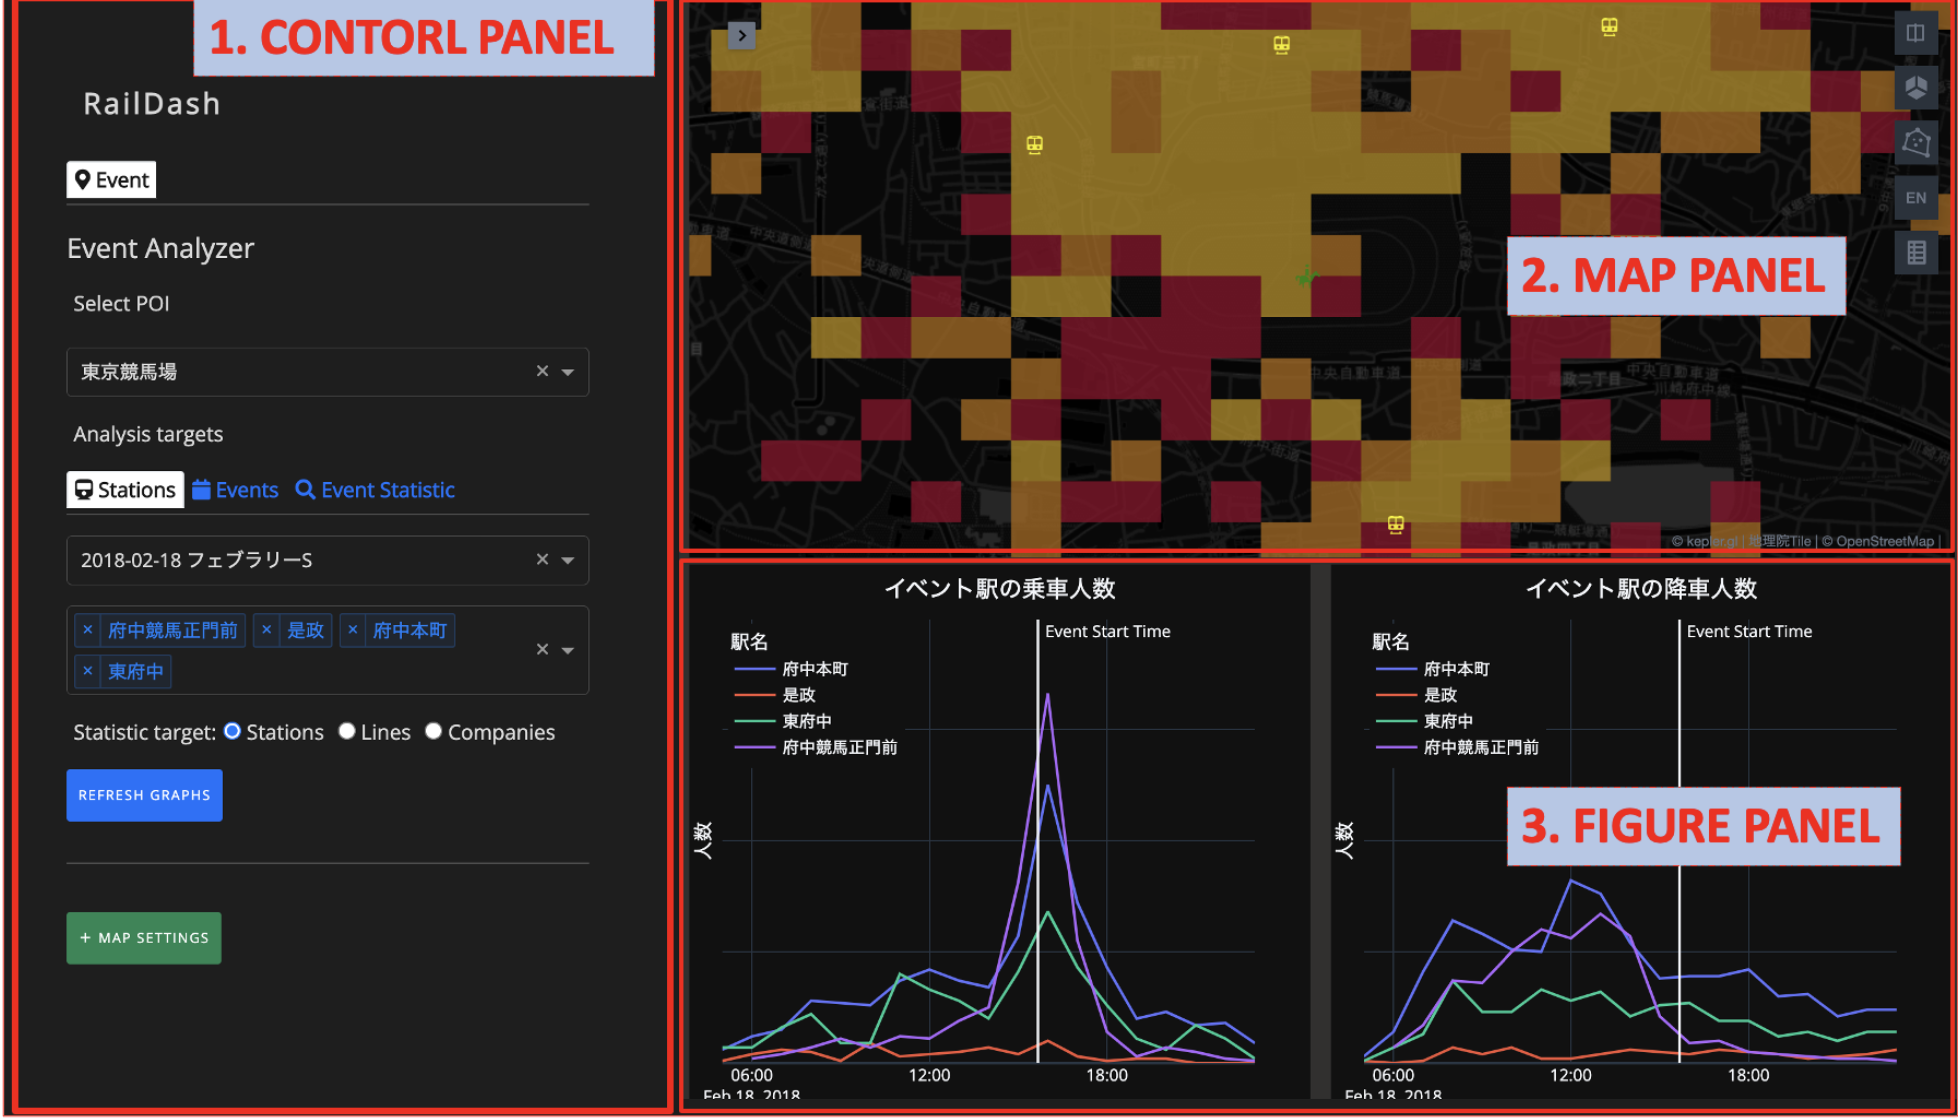
\includegraphics[width=.5\linewidth]{content/00_assets/raildash.png}
    \label{fig_raildash}
\end{figure}

Die Qualität des Dashboards ist nebst anderen Faktoren wie Ben Shneidermanns «8 goldenen Regeln» \parencite{golden_rules_dashboard} auch stark von der Datenqualität und insbesondere der korrekten Wahl der passenden Visualisierung abhängig. Wird eine schlechte Visualisierung gewählt, resultiert dies in einem schlechten Dashboard. Es folgt daher ein Überblick über etablierte Visualisierungen und deren Anwendungsfälle. Die zwei wichtigsten Datentypen in Verkehrsdaten sind \textbf{räumliche} sowie \textbf{zeitliche} Daten. 

\subsection{Zeitliche Visualisierungen}
Bei den \textit{zeitlichen} Daten wird gemäss Chen et al. zwischen \textbf{linearen} und \textbf{periodischen} Zeitintervallen unterschieden. \textit{Lineare Zeitintervalle} haben einen definierten Start und Endpunkt. Solche Zeitintervalle beschreiben mittels Höhen- und Tiefpunkte, wie sich die Daten über die Zeit ändern. Für lineare Zeitintervalle werden häufig Liniendiagramme verwendet. Liniendiagramme sind einfach zu interpretieren, jedoch nicht die geeignete Wahl, wenn es um die Darstellung von \textit{mehreren Variablen} geht (Visual Clutter Problematik). Nebst Liniendiagramme bieten sich auch Theme Rivers an \parencite[S. 2973]{survey_traffic_data_visualization_2015}.

\textbf{Periodische Zeitintervalle} beschreiben wiederkehrende Prozesse mit einem bestimmten Intervall (Wochentage, Monate etc.). Für solche Daten eignen sich besonders radiale Visualisierungen. In Abbildung \ref{fig_radial_layout} wird ein Tag als Kreis visualisiert, wobei die Farbe der Kreissegmente die Verkehrsauslastung darstellt \parencite[S. 2973 - 2974]{survey_traffic_data_visualization_2015}.

\begin{figure}[H]
    \caption{Radiale Visualisierung \parencite[S. 5]{radial_layout_t_watcher}}
    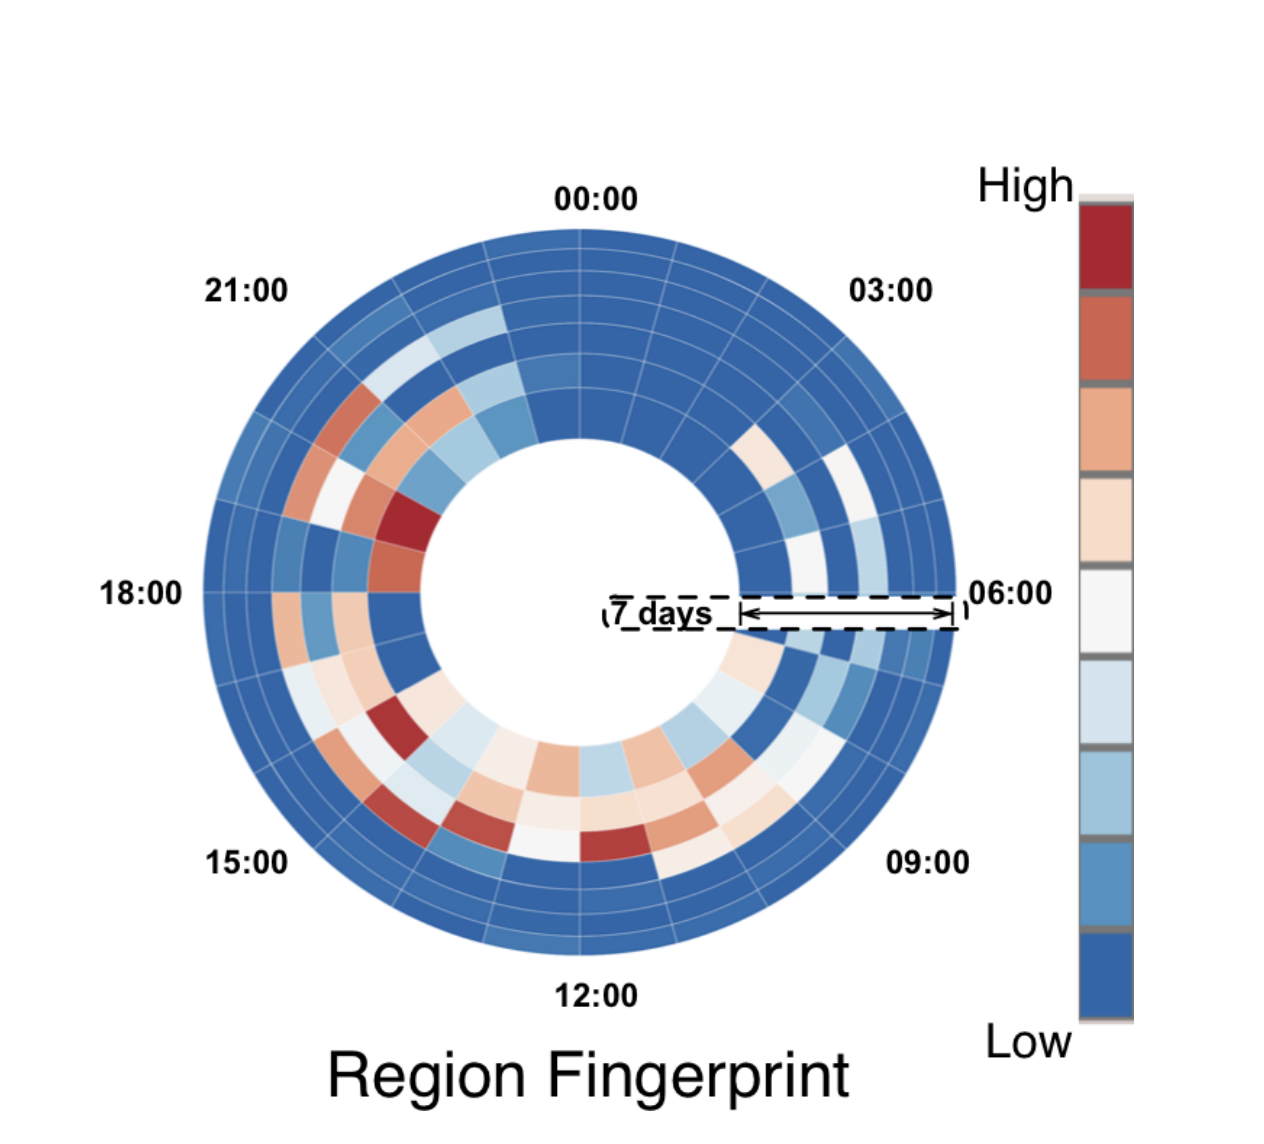
\includegraphics[width=.5\linewidth]{content/00_assets/radial_layout.png}
    \label{fig_radial_layout}
\end{figure}

\subsection{Räumliche Visualisierungen}
Räumliche Eigenschaften lassen sich gemäss Chen et al. in \textbf{punktebasierte, linienbasierte}, sowie \textbf{regionenbasierte} Visualisierungen einteilen \parencite[S. 2974 - 2975]{survey_traffic_data_visualization_2015}.

\textbf{Punktbasierte Visualisierungen} repräsentieren die Daten als Punkte. Über die visuellen Variablen Grösse und Farbe können dem Nutzer weitere Aspekte vermittelt werden. Der Vorteil von punktbasierten Visualisierungen besteht darin, dass der Nutzer den Zustand aller Objekte gleichzeitig beobachten kann. Zudem können Punktvisualisierungen dabei helfen, stark belastete Bereiche (Cluster) hervorzuheben. Jedoch besteht bei grossen Datenmengen die Gefahr von Visual Clutter. Eine Möglichkeit, um Visual Clutter zu vermindern, ist die Verwendung von Heatmaps in Kombination mit dem \textbf{\acrfull{kde}} Algorithmus (siehe Abbildung \ref{fig_heatmap_kde}).

\begin{figure}[H]
    \caption{Heatmap-Visualisierung mit KDE-Algorithmus \parencite{vait_system}}
    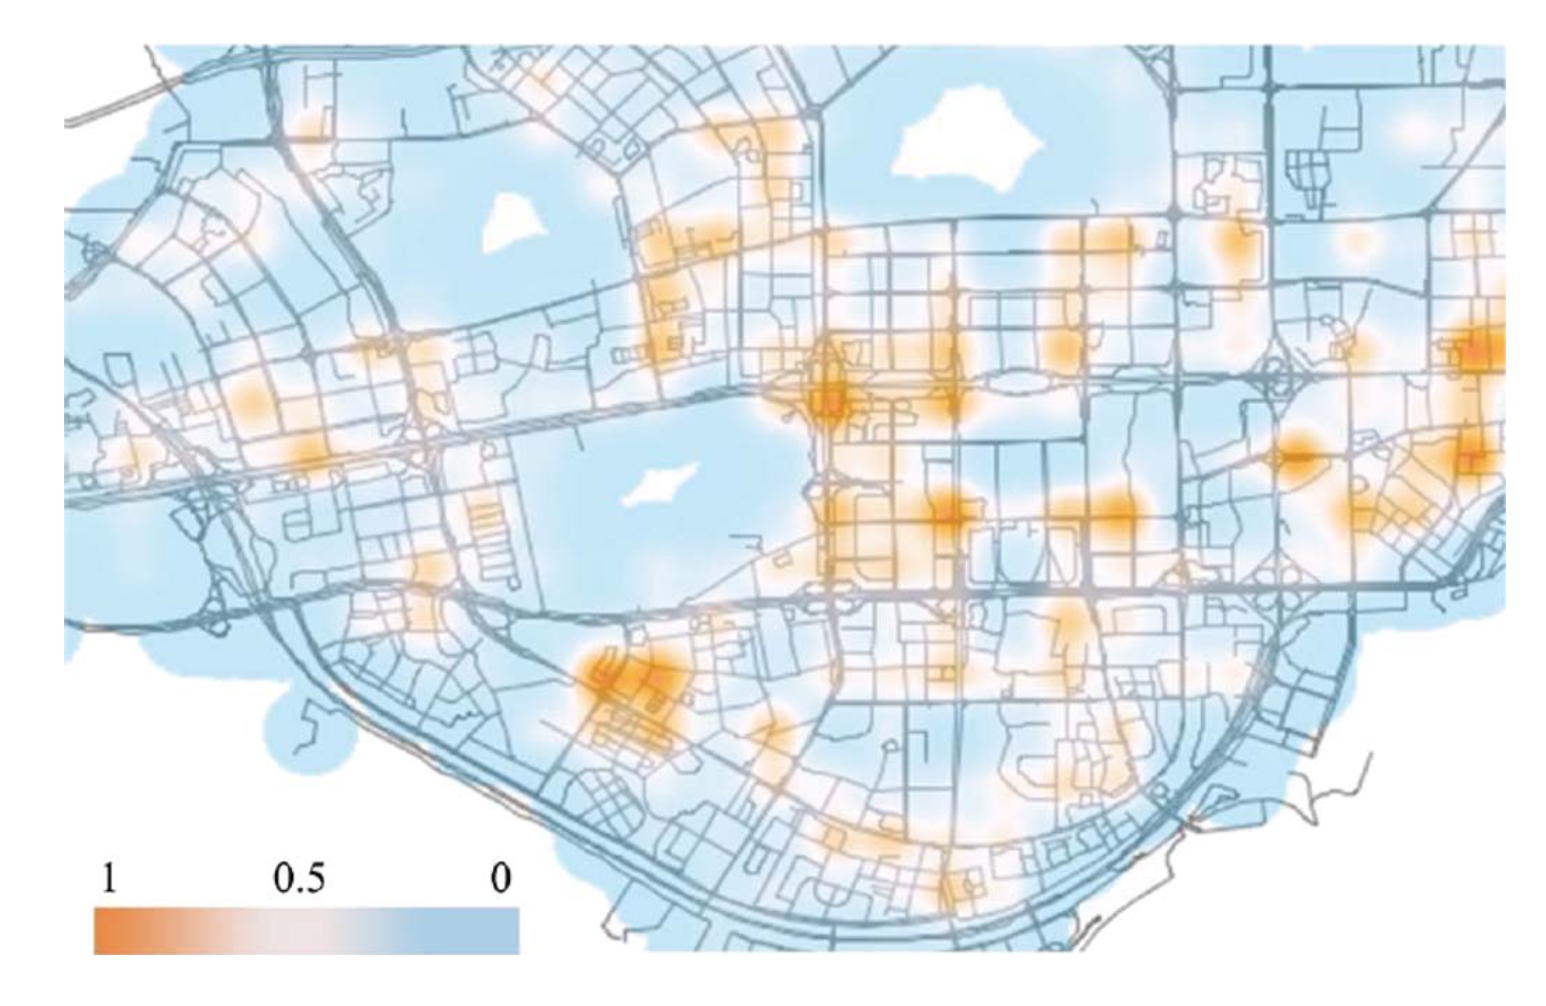
\includegraphics[width=.5\linewidth]{content/00_assets/heatmap_kde.png}
    \label{fig_heatmap_kde}
\end{figure}

\textbf{Linienbasierte Visualisierungen} werden eingesetzt, um den Fluss von Verkehrsnetzwerken zu veranschaulichen. Im Falle von Zugnetzwerken können etwa die Streckennetze als einzelne Linien (Trajektorien) dargestellt werden, wobei die Dicke der Linie die Auslastung und die Farbe die Verspätung visualisieren könnte. Bei einer grossen Anzahl von Linien entsteht auch wiederum Visual Clutter. Ein bewährter Lösungsansatz für dieses Problem ist das sogenannte «Edge Bundling». Hierbei werden ähnliche Linien zu einem «Bündel» zusammengefasst \parencite[S. 2974 - 2976]{survey_traffic_data_visualization_2015}. Eine weitere Möglichkeit besteht darin, anstelle von Edge Bundling den \acrshort{kde} Algorithmus auf die Trajektorien anzuwenden (siehe Abbildung \ref{fig_line_kde}).

\begin{figure}[H]
    \caption{Linienbasierte Visualisierung mit KDE-Algorithmus \parencite[S. 7]{streaming_data_kde}}
    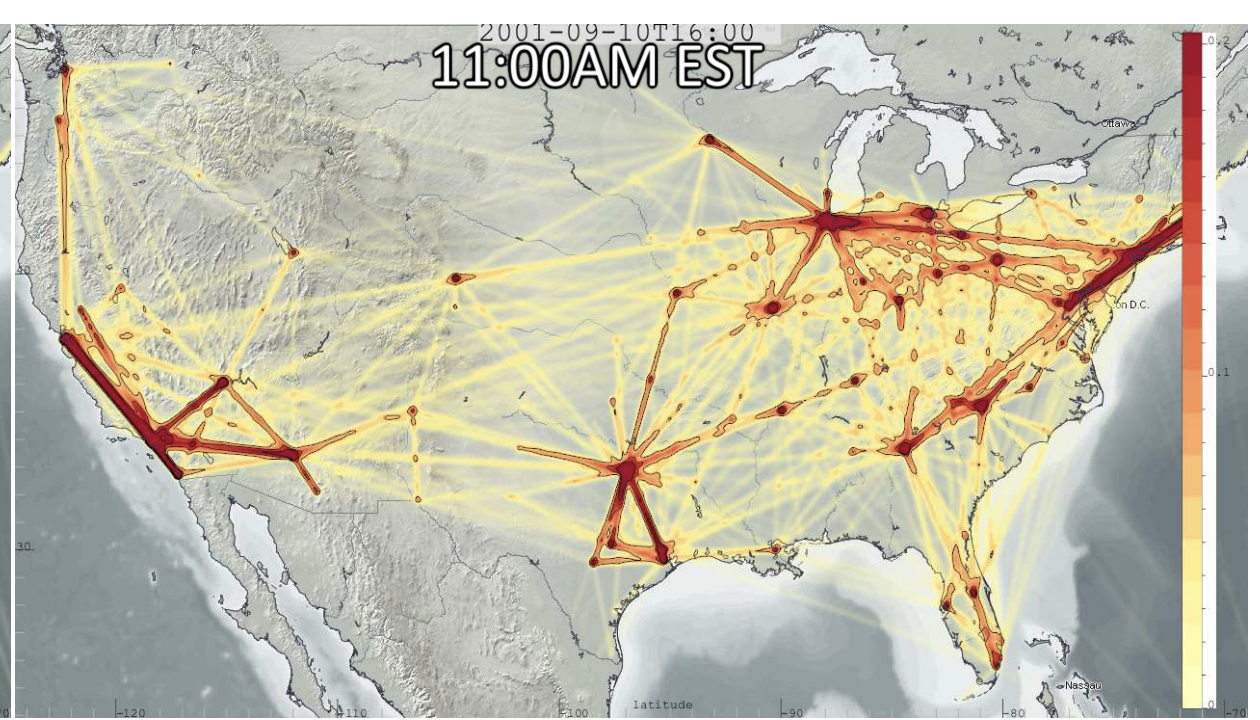
\includegraphics[width=.5\linewidth]{content/00_assets/line_visualization_kde.png}
    \label{fig_line_kde}
\end{figure}

\textbf{Regionalbasierte Visualisierungen} erlauben es gemäss Chen et al. Makro-Patterns in Verkehrsdaten zu visualisieren, beispielsweise wie sich die Zugverspätungen pro Region unterscheiden. Sie sind jedoch nicht geeignet, um Mikro-Patterns von einzelnen Zügen zu visualisieren \parencite[S. 2976]{survey_traffic_data_visualization_2015}.

\section{Erkennung von visuellen Mustern}
TODO

\section{Grafstrukturen}
TODO


